\section{Building MCG and FPG}
    \label{s:building graphs}
\subsection{Maximal Connectivity Graph}
    \label{ss:MCG}
    To construct the maximal connectivity graph, we assume that a set of codes, global inputs, and objectives and constraints (collectively called global outputs) are provided. 
    The codes are represented by analysis block graphs ((ABGs?)) $A_i=(V_{A_i},E_{A_i}), \ i\in I$, where $m$ is the number of codes and $I=\{1,2,\ldots,m\}$. 
    The global inputs are represented as a set of variable nodes $V_\txt{in}$, and the global outputs are represented by a set of variable nodes $V_\txt{out}$. 
    We assume that $V_\txt{in}$, $V_\txt{out}$, and each $A_i$ are given, and that any potential connection between variables is given in the form of connection edges in the set $C_M$. 
    Then we may construct the maximal connectivity graph $M=(V_M,E_M)$ as
    \begin{IEEEeqnarray*}{rCl}
    V_M & = & V_\txt{in} \cup V_\txt{out} \cup \left( \bigcup_{i \in I} V_{A_i} \right), \\
    E_M & = & C_M \cup \left( \bigcup_{i \in I} E_{A_i} \right),
    \end{IEEEeqnarray*}
    The MCG $M$ is uniquely determined by the given set of analysis blocks, the required outputs, and the given global inputs. 
    In the cases where the set of global inputs is not known a priori, the process of obtaining the FPG will reveal the required inputs, as discussed subsequently.

\subsection{Fundamental Problem Graph}
    \label{ss:FPG}
    We now define the fundamental problem graph $F=(V_F,E_F)$ as a directed graph meeting the following conditions, which are explained subsequently,
    \begin{enumerate}
    \item[(1)] $F \subset M$ and $V_\txt{out} \subset V_F$
    \item[(2)] $\displaystyle{\forall i \in I, \txt{ if } F \cap A_i \neq \emptyset \txt{ then } A_i \subset F}$
    \item[(3)] $\displaystyle{\forall v \in V_F \txt{ with } t_\txt{node}(v) = \txt{`variable,'} \  \txt{deg}_l^-(v) \leq \txt{deg}^-(v) \leq \txt{deg}_u^-(v)}$
    \item[(4)] $\displaystyle{\forall v \in V_F \txt{ there exists a reverse path } P \subset R_F \txt{ from } x \txt{ to } v \txt{ with } x\in V_\txt{out}}$
    \end{enumerate}
    %The set $I_F$ is an index set containing the indices of the analysis blocks in $F$ and it may only include the analysis blocks $A_i$ that meet requirements (2) and (6). 
    %Requirement (2) stipulates that each analysis blocks in $F$ must have at least one local output that is being used. 
    %Requirement (3) stipulates that only the global inputs that are being used should be included. 
    %Requirements (4) and (5) provide the construction of the sets of nodes and edges, respectively. 
    Requirement (1) asserts that only the nodes and edges provided by the maximal connectivity graph can be used in the fundamental problem graph and that every global output must be included. 
    Requirement (2) requires that each analysis block must be entirely present or entirely absent. 
    Requirement (3) stipulates that the number of edges directed into each variable node must be within the lower and upper in-degree limits; 
    if $\txt{deg}^-(v) < \txt{deg}_l^-(v)$ the node is a \emph{hole}, and if $\txt{deg}^-(v) > \txt{deg}_u^-(v)$ the node is a \emph{collision}.
    Lastly, requirement (4) ensures that only the nodes that are being used are included in the FPG by requiring that for every node a reverse path exists from at least one global output to that node. 
    The reverse graph $R_F$ is obtained from $F$ by simply switching the orientation of every edge in $E_F$.

    %The set $C_F$ is a set containing connection edges representing connections. Since $C_M$ is the set of all potential connections, we must have $C_F \subset C_M$. 
    %While no other conditions are explicitly stated for $C_F$, requirement (6) is actually a requirement on both $I_F$ and $C_F$.

\subsection{Obtaining the Fundamental Problem Graph}
    \label{ss:obtaining FPG}
    In general, there may be multiple different graphs that satisfy the FPG conditions in Sec.~\ref{ss:FPG}, though there may be none at all. 
    Here, we describe a process for obtaining an FPG by starting with the MCG and disconnecting connection edges until the FPG conditions are met. 
    Then the problem is reduced to deciding which connection edges to remove.

((describe pruning as a subroutine enforcing step 4 and then step 2))

    \begin{description}
    \item[Subroutine: Pruning] 
        Given a digraph $G_1 = (V_1,E_1)$, let the subroutine denoted as $P_\txt{prune}$ operate on $G_1$ to produce a digraph $G_2 = (V_2,E_2)$ that satisfies requirements (2) 
        and (4), and write $G_2 = P_\txt{prune} ( G_1 )$. 
        This is accomplished by first creating the reverse graph of $G_1$, $R = (V_1,E_R)$. Then adding a new node $x$ to $V_R$ and adding edges directed from this node to each of the global outputs, i.e.,
    \begin{equation}
        \forall y \in V_\txt{out}, (x,y) \in E_R
    \end{equation}
        The set of nodes that may be reached from the global outputs is constructed as
    \begin{equation}
        U = \{ n \in V_1 \st \exists P \txt{ a path from $x$ to $n$}, \ P \subset R \}.
        \end{equation}
        The list of analysis blocks with at least one node that may be reach is constructed as
        \begin{equation}
        I_1 = \{ i \in I \st V_{A_i} \cap U \neq \emptyset \}
        \end{equation}
        The set of nodes to remove is
        \begin{equation}
        N = \{ v \in V_1 \st v \in V_{A_i} \txt{ for } i \in I_1, \txt{ or } v \in V_\txt{in}\setminus U \},
        \end{equation}
        which means that $N$ is composed of unused analysis block nodes and unused global input nodes. Then the new set of nodes is created as
        \begin{equation}
        V_2 = V_1 \setminus N,
        \end{equation}
        and edges involving the removed nodes are also deleted
        \begin{equation}
        E_2 = E_1 \setminus \{ (a,b) \st a \in N \txt{ or } b \in N  \}.
        \end{equation}
        The set of connection edges can be obtained as
        \begin{equation}
        C_2 = \{(x,y) \in V_{2} \st \sim(x \in V_{A_i} \txt{ and } y \in V_{A_i} \txt{ for some } i \in I_1)\},
        \end{equation}
        which means $C_2 \cap V_{A_i} = \emptyset  \ \forall i \in I_1$, and $E_2 = C_2 \cup \left( \bigcup_{i \in I_1} E_{A_i} \right)$. 

    \item[Step 1: Holes] 
        The first step is to detect holes and disconnect the connection edges following them. 
        These connection edges are removed because they represent variables which cannot be determined because the analysis function does not have adequate inputs. 

        To start, the an initial graph is created as a pruned copy of the MCG
        \begin{equation}
        F_0 = P_\txt{prune}(M),
        \end{equation}
        where $F_0 = (V_{F,0},E_{F,0})$, and $C_{F,0}$ is also obtained as described. 
        The set of variable nodes which are holes is created as
        \begin{equation}
        H = \{v \in V_{F,0} \st t_\txt{node}(v) = \txt{`variable'} \txt{ and } \txt{deg}^-(v) < \txt{deg}_l^-(v) \},
        \end{equation}
        which is the set of variable nodes with fewer incoming edges than are allowed by the lower in-degree limit.
        Then the updated set of edges is created by removing the edges preceding or succeeding the analysis block:
        \begin{equation}
        C_{F,1} = C_{F,0} \setminus \{(x,y) \in C_{F,0} \st x \in V_{A_i} \txt{ or } y \in V_{A_i}, \txt{ and } H\cap V_{A_i} \neq \emptyset \},
    \end{equation}
    %deg-v is now recaculated for the new C. 
    and this step is demonstrated by Fig.~\ref{f:hole}. Because removing these edges can create new holes, this step must be repeated until no more holes are found.
        If this step every finds a global output to be a hole, meaning $V_\txt{out} \cap H \neq \emptyset$, then the algorithm stops because an FPG cannot be obtained. 
        Otherwise, it is guaranteed that an FPG can be obtained.
    \begin{figure}[htb!]
        \begin{center}
        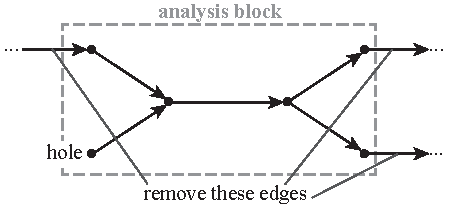
\includegraphics[width=3in]{images/analysis_block_hole}
        \end{center}
        \vspace{-20pt}
    \caption{Example variable node indicating a hole.}
    \label{f:hole}
    \end{figure}

    \item[Step 2: Collisions] 
        The second step is to detect collisions and to then disconnect enough connection edges so that the collisions are resolved. 
        The set of variable nodes which contain collisions is created as
    \begin{equation}
    S_\txt{nodes} = \{v \in V_M \st t_\txt{node}(v) = \txt{`variable'} \txt{ and } \txt{deg}^-(v) > \txt{deg}_u^-(v) \}.
    \end{equation}
    For each collision node we can construct a set contained the edges directed in. The set containing all of these sets is constructed as
    \begin{equation}
        S_\txt{edges} = \big \{ \{(x,y) \in E_M\} \ \big| \ y \in S_\txt{nodes} \big \}
    \end{equation}
    Let $J=\{1,2,\ldots,|S_\txt{edges}|\}$ be an indexing set for $S_\txt{edges}$ such that each $S_{\txt{edges},j}$ corresponds to a set in $S_\txt{edges}$ for $j \in J$. 
    An example collision is shown in Fig.~\ref{f:collision} to indicate the definition of $S_{\txt{edges},j}$. 
    We can assume that $J$ also indexes $S_\txt{nodes}$ because there is a one--to--one correspondence between the elements in $S_\txt{nodes}$ and the elements in $S_\txt{edges}$ (which are sets). 
    Then we may construct sets of edges as
    \begin{equation}
    B_j = \big \{e_k \in S_{\txt{edges},j} \st k \in \{1,2,\ldots,K\} \txt{ with } K \leq \txt{deg}_u^-(v_j) \big \}, \ j \in J,
    \end{equation}
        which means that each set $B_j$ is constructed from the set $S_{\txt{edges},j}$ by taking only as many edges as are allowed by the upper in--degree limit of $v_j$. 
        The construction of each $B_j$ corresponds to making a decision on which edges to include and which edges not to include. Then let
    \begin{equation}
    C_{F,2} = \{ e \in C_{F,1} \st e \in B_j \txt{ for some } j \in J\},
    \end{equation}
    \begin{equation}
    E_{F,2} = E_M \setminus (C_M \setminus C_{F,2})
    \end{equation}
    and
    \begin{equation}
    F_2 = (V_M,E_{F,2})
    \end{equation}
    \begin{figure}[htb!]
        \begin{center}
        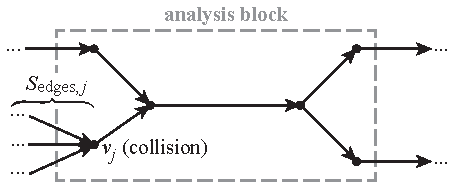
\includegraphics[width=3in]{images/analysis_block_collision}
        \end{center}
        \vspace{-20pt}
    \caption{Example variable node indicating a collision.}
    \label{f:collision}
    \end{figure}

    \item[Step 3: Finalize] 
        The third and final step is to prune the graph one last time
    \begin{equation}
        F = P_\txt{prune}(F_2),
    \end{equation}
        and $F = (V_F,E_F)$.
        The indices of the used analysis blocks can then be found as
    \begin{equation}
        I_F = \{ i \in I \st A_i \cap F \neq \emptyset \}
    \end{equation}
%       \begin{
%       \begin{equation}
%       I_F =  \{i \in I \ | \ \exists v \in V_{A_i} \txt{ such that }  t_\txt{node}(E_{F,2}^{-1}(v))=\txt{`model'} \txt{ and } \txt{deg}^+(v) > 0 \},
%       \end{equation}
%       where the degree is calculated with respect to $F_2$. 
%       This set excludes both the analysis blocks that were unused in the original MCG and those that became unused in step 1 or step 2.
%
%       The set of used global inputs is constructed as
%       \begin{equation}
%       V_{\txt{in},F} = \big\{v \in V_\txt{in} \ \big| \ |\{(x,y) \in E_{F,2}(v) \st y \in V_{A_i} \txt{ for } i \in I_F  \}| > 1 \big\},
%       \end{equation}
%       which requires that at least two edges directed out of the nodes in $V_{\txt{in},F}$ must be to the analysis blocks indexed by $I_F$.
%
%       Finally, the set of nodes and edges describing a fundamental problem graph is given by
%       \begin{equation}
%       V_F = V_{\txt{in},F} \cup V_\txt{out} \cup \left( \bigcup_{i \in I_F} V_{A_i} \right),
%       \end{equation}
%       \begin{equation}
%       C_{F} = \{ (x,y) \in C_{F,2} \st x,y \in V_F\},
%       \end{equation}
%       \begin{equation}
%       E_F = C_F \cup \left( \bigcup_{i \in I_F} E_{A_i} \right),
%       \end{equation}
%       \begin{equation}
%       F = (V_F,E_F).
%       \end{equation}

    \end{description}

This process will always provide an FPG if one exists. If an FPG does not exist, this process will reveal the limiting factors preventing a valid formulation.